% Template source: https://www.overleaf.com/11321160gbgqghnxhmwj#/42733219/
%++++++++++++++++++++++++++++++++++++++++
% Don't modify this section unless you know what you're doing!
\documentclass[%
	 aps,%
	 prl,%
	 a4paper,%
	 amsmath,amssymb,%
	 preprint,%
	 reprint,%
	%author-year,%
	%author-numerical,%
]{revtex4-1}
% Users of the {thebibliography} environment or BibTeX should use the
% scicite.sty package, downloadable from *Science* at
% www.sciencemag.org/about/authors/prep/TeX_help/ .
% This package should properly format in-text
% reference calls and reference-list numbers.

%\usepackage{scicite}

% Use times if you have the font installed; otherwise, comment out the
% following line.

%\usepackage{times}

% The preamble here sets up a lot of new/revised commands and
% environments.  It's annoying, but please do *not* try to strip these
% out into a separate .sty file (which could lead to the loss of some
% information when we convert the file to other formats).  Instead, keep
% them in the preamble of your main LaTeX source file.


% The following parameters seem to provide a reasonable page setup.

% RK imports:============================
\usepackage{silence}
\WarningFilter{revtex4-1}{Repair the float}
\usepackage{graphicx,float,wrapfig}
\usepackage{xcolor}
\usepackage{amsmath}
\usepackage[left,switch,mathlines]{lineno}
\setlength\linenumbersep{1cm}\modulolinenumbers[2]

% For arXiv formatting
\usepackage[top=1.2cm, bottom=1.0cm, left=1.0cm, right=1.0cm]{geometry}

\usepackage{graphicx}% Include figure files
\usepackage{dcolumn}% Align table columns on decimal point
\usepackage{bm}% bold math

%\usepackage{biblatex}

%\usepackage{multibib}
%\newcites{SOMs}{Additional References}

\newcounter{firstbib}

\usepackage[colorlinks=true,%
			allcolors=blue,bookmarks=false,pdfusetitle]{hyperref}
\usepackage{url}
% =======================================

%\topmargin 0.0cm
%\oddsidemargin 0.2cm
%\textwidth 20cm 
%\textheight 21cm
%\footskip 1.0cm


%The next command sets up an environment for the abstract to your paper.

%\newenvironment{sciabstract}{%
%\begin{quote} \bf}
%{\end{quote}}


% If your reference list includes text notes as well as references,
% include the following line; otherwise, comment it out.

%\renewcommand\refname{References and Notes}

% The following lines set up an environment for the last note in the
% reference list, which commonly includes acknowledgments of funding,
% help, etc.  It's intended for users of BibTeX or the {thebibliography}
% environment.  Users who are hand-coding their references at the end
% using a list environment such as {enumerate} can simply add another
% item at the end, and it will be numbered automatically.

\newenvironment{comment}{\textcolor{blue}}

\newenvironment{reply}{\textcolor{green}}

\newenvironment{todo}[1]{{\textcolor{red}#1}}

\newcounter{lastnote}
\newenvironment{scilastnote}{%
\setcounter{lastnote}{\value{enumiv}}%
\addtocounter{lastnote}{+1}%
\begin{list}%
{\arabic{lastnote}.}
{\setlength{\leftmargin}{.22in}}
{\setlength{\labelsep}{.5em}}}
{\end{list}}

\newcommand{\Rev }[1]{{\color{blue}{#1}\normalcolor}} % Revision
\newcommand{\Com}[1]{{\color{red}{#1}\normalcolor}} %Comment
\newcommand{\rev }[1]{{\color{blue}{#1}\normalcolor}} % revision
\newcommand{\com}[1]{{\color{red}{#1}\normalcolor}} %comment
\newcommand{\mjd}[1]{{\color{green}{#1}\normalcolor}} %Comment
%++++++++++++++++++++++++++++++++++++++++


\begin{document}

\title{Observation of Quantum Depletion in the Momentum Distribution from a Magnetically Trapped Bose-Einstein Condensate}

\author{J.~A.~Ross, D.~K.~Shin, B.~M.~Henson, S.~S.~Hodgman, A.~G.~Truscott}

\affiliation{Laser Physics Centre,Research School of Physics and Engineering,\\Australian National University, Canberra 0200,~Australia}

\date{\today}

\begin{abstract}
%\textcolor{blue}{In below, fixes are red and comments are blue. Use the environments fix\{\} and comment\{\} respectively to add.}

% Quantum depletion is an interesting many-body phenomenon wherein repulsive interactions between atoms modify the single-particle momentum eigenstates of a Bose-Einstein condensate.  A recent experiment \cite{Chang2016} observed quantum depletion in a Bose-condensed gas of helium atoms released from an optical dipole trap.  However, current theoretical understanding \cite{Qu2016} is that the depletion should not be observable after trap switch off in the presence of interactions.  To attempt to resolve this problem, we follow a similar method to \cite{Chang2016}, where we observe quantum depletion of a Bose-Einstein condensate released from a magnetic trap, evident as a long tail at large momenta with the density scaling as $k^{-4}$.  The values of the Tan contact constant we measure are slightly larger than those predicted by local density theory, although the discrepancy is smaller than for the results reported in \cite{Chang2016}.  Our observation suggests that the results seen here and in \cite{Chang2016} are not an experimental anomaly, but rather demand deeper theoretical investigation to determine why the tails survive the trap switch-off and subsequent expansion.
\end{abstract}

\maketitle


\section{Introduction}
% \fix{
% \begin{itemize}
% 	\item Address plot comments
% 	\item Add fill in missing parameters
%     \item Discuss fit method more carefully
% \end{itemize}
% }
A Bose-Einstein condensate (BEC) forms when a system of bosons is cooled below a critical temperature, where the majority of atoms occupy the ground state of the system.  At non-zero temperature, the condensate will be depleted by thermal excitations, where some atoms occupy higher energy states with occupation probabilities following a Bose-Einstein statistics/todo{MB distribution?}.  However, even at absolute zero, the condensate will still be depleted by quantum fluctuations, a phenomenon known as quantum depletion.  The spectrum of fluctuations in the quasiparticle vacuum gives rise to an asymptotic momentum distribution that follows a $k^{-4}$ power law\cite{Qu2016}.

A recent experiment \cite{Chang2016} was able to see evidence of quantum depletion in the large $k$ tails of an interacting BEC released from an optical dipole trap, using the high-resolution and large dynamic range of detection offered by ultracold metastable helium atoms (He*) \cite{Vassen2012}.  A separate experiment on a strongly interacting BEC in a uniform potential probed with Bragg scattering showed that the depletion could be tuned with the interaction strength \cite{Lopes2017}.\todo{Complete experimental review}

According to current theory however, the quantum depletion seen in \cite{Chang2016} is not expected to be observed, as the interactions between atoms should cause the $k^{-4}$ tails to adiabatically vanish during the expansion after trap switch off \cite{Qu2016}. 
During the expansion, which is taken to be hydrodynamic, the contact parameter tends to zero, which eliminates the depletion tail for sufficiently long expansions.  This viewpoint was supported by an earlier experimental result that failed to observe the tails \cite{Makotyn2014}.  However, it is unclear whether the high momentum tails, which are by definition fast moving, are in fact accurately described by this model or if their shorter interaction time with the high density region of the BEC (in a semi-classical picture) means they do in fact survive the expansion.  
To help resolve this discrepancy, we have conducted a similar experiment to \cite{Chang2016} looking at the momentum tails of a BEC of He* released from a magnetic trap and detected after a long time of flight.  

%\comment{Re-reading Qu et al the argument seems to be:
%Qu et al \cite{Qu2016} claim that the depleted fraction should not be visible in the asymptotic momentum distribution by the following logic: Given the contact parameter is proportional to the integral of the squared density, one can use the hydrodynamic expansion of the BEC to show that the contact parameter tends to zero during expansion. This may be true for the expanding condensate, but (semiclassically thinking) the high-momentum particles would actually leave, hence decouple from, the condensate, and remain visible in the asymptotic density distribution}

\section{Methods}
Our experiments start with a condensate of helium atoms in the $M_J = +1$ state of the metastable $2^3 S_1$ manifold in a BiQUIC magnetic trap \cite{Dall2007}. The trap is switched off in $\sim 100\mu s$ and the atoms allowed to fall 848mm, where they are detected with a multi-channel plate and delay line detector \cite{Manning2010}.  To reduce the detector saturation, 2ms after trap switch-off we transferred approximately 43\% of the condensate into the magnetically insensitive $M_J=0$ state by applying a chirped sine wave, swept from 1.6 to 2.6 MHz in 1ms, while a DC magnetic field remained on to preserve the Zeeman splitting between $M_J = \{0,\pm 1\}$ states.  A magnetic field gradient is switched on 5ms after the state transfer pulse, which ensures the magnetically sensitive $M_J = \pm 1$ states are deflected enough to miss the detector. 

After release from the trap the atoms expand ballistically into the far-field regime, where their position on the detector corresponds to their momentum after trap release by $\textbf{k} = m\textbf{r}/\hbar t_{tof}$, where $t_{tof}$ is the fall time to the detector. Therefore we can reconstruct the far-field momentum distribution $n^*(\textbf{k})$ from our detector data. The observed momentum profile $n^*(\textbf{k})$ cannot be identified completely with the in-trap momentum distribution $n_0(\textbf{k})$ as repulsive interatomic forces distort the profile immediately after release from the trap. \todo{Is this basically the argument for why we see the increased depletion?}
%\comment{[Has anyone actually modeled/measured this?]} 
% As in \cite{Chang2016} we find the large-$\textbf{k}$ momentum distribution is isotropic, unlike the in-trap mean-field interactions, and conclude that the extreme momenta are not strongly affected by the mean-field. 
A typical condensate profile shown in Fig. \ref{k_profile}.  Structure is visible over five orders of magnitude in density, comprised of the condensed, thermal, and depleted fraction before the signal drops below the dark-count background noise. There is some saturation evident around the low momentum values due to the high atom flux during BEC impact, however this part of the histogram is not used for the analysis. 

The quantum depletion is extracted following a similar procedure to Chang et al \cite{Chang2016} to fit the data outside the central BEC with a functional form that includes contributions from the thermal fraction, depleted fraction, as well as a constant background due to detector background counts.  We transform the histogram data by $n'(\textbf{k}) = |\textbf{k}|^4\times n^*(\textbf{k})$ and fit with the function $n_{fit}(k)\times k^4$, where
$$
n_{fit}(k) = \frac{N_{th}g_{3/2}exp(-k^2 \lambda_{dB} ^2 /4\pi)}{1.202(2\pi/\lambda_{dB})^3} + \frac{C}{(2\pi)^3 k^4} + const, 
$$
with four free parameters: $N_{th}$ the number of thermal atoms, $\lambda_{dB} = h/\sqrt{2\pi m k_B T}$ the thermal de Broglie wavelength, $const$  a constant to account for the detector background count rate, and $C$ is the scale of the fitted power law assumed to correspond to the Tan contact parameter. In the local density approximation, $C \approx C_{LDA} = \int d\textbf{r} [16\pi^2 \rho^2(\textbf{r},t)a^2]$, where $a$ is the scattering length and $\rho$ the atomic density. 
\todo{Verify fitting is faithful estimator; examine bias and stability for unconstrained powers}
%\comment{[Keeping the power law exponent as a free parameter, rather than fixing it at 4, has not so far been successful]} 
% The fit is shown in Fig. \ref{k_profile} as a green line, and is seen to agree with the data well.  This good agreement and fit robustness is due to each of the three contributions dominating at a distinctly separate range of $k$ values.

To investigate the behaviour of the depletion over a wide range of system parameters, we used traps with two different configurations as well as different total atom numbers:  One trap configuration characteristic frequencies $ \sim 2\pi\cdot (312,312,52)$ and the other with $\sim 2\pi\cdot (476,476,66)$ Hz. Since for these experiments a precise knowledge of the total atom number and trap frequency is important, we developed an experimental procedure to regularly calibrate the trapped population and trapping frequency at regular intervals throughout each experimental run, using a procedure that avoids detector saturation to measure the atom number (see supplementary material).  We varied total atom number  between 1 and $5\times 10^5$ atoms per condensate by varying the endpoint of the evaporative cooling ramp.
The depletion is a feature of the condensed atoms in the ground state, and expected to be unaffected by the changes in temperature.   \todo{However, the contact is temperature-dependent, how important is it expected to be?} As shown in Fig \ref{C_inf}, the quantum-depleted population is affected by the trap frequencies and population only inasmuch as they determine the peak density.
%We operated our traps in a constant DC bias field to maintain the Zeeman splitting between the $M_J$ states, which is required for the RF transfer sequence detailed below. Our measurements were made by a delay-line detector placed 848mm below the condensate, upon which the condensate lands after expanding into the far-field regime in free-fall through the vacuum chamber. with a magnetically trapped BEC and additional calibration of the condensate population and density.

\begin{figure}[b]
\centering
\includegraphics[width=0.5\textwidth]{profile_update.png}
\caption{
A typical far-field momentum profile taken for $N_0 = 5.8(2)\times 10^5$ atoms at $\omega/2\pi = (312,312,52)$ Hz. Purple circles are the average of $\sim 3000$ shots. The green line is a fit to the thermal and depleted fractions, taking into account the detector background count rate.  %\com{[might be better to show data as 3 lines, mean and std. Remove space between $mu$ and m in unit.] }
}
\label{k_profile}
\end{figure}

\section{Results}

%Across all datasets, we find that fitting procedure outlined above yields a power law exponent of $\alpha = \fix{-X.X(X)}$ \comment{Actually, I only fitted with $\alpha$=4. We should chat about this method in detail}. By analysis of residuals, the fit errors appear random. \comment{This is a very weak claim - needs bolstering for final paper, or omission here}. This suggests that the profile consists of a thermal fraction, the background count contribution, and a quantum depleted fraction that is consistent with a power law with exponent \fix{X.X()}. 

According to theoretical predictions based on the local density approximation \cite{Chang2016}, the contact constant $C_{LDA}$ of the depleted fraction should vary linearly with the peak condensate density $n_0$.  This was found in previous experiments\cite{Chang2016}, although their scaling factor was out by a factor of $\sim$6.5. In Fig. \ref{C_inf}, we plot our measured values of $C$ and $n_0$, identifying the fit parameter $C$ with the contact constant $C_{LDA}$. A linear fit to the contact constant variation finds a gradient approximately 1.6 times more than the theory predicts, closer to theory than the previous measurement \cite{Chang2016} (dotted line in Fig. \ref{C_inf}. This may suggest that there are physical effects beyond the local density approximation that need to be accounted for.  

\begin{figure}[b]
\centering
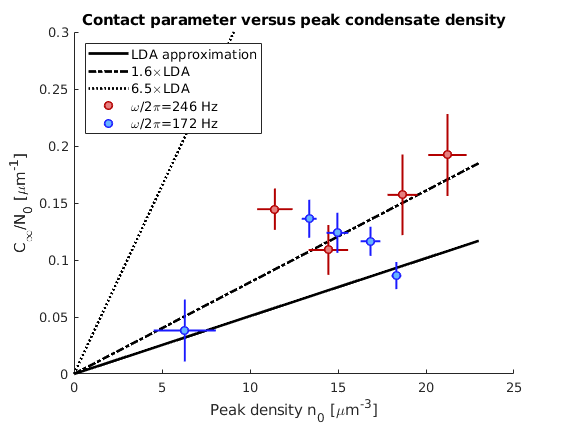
\includegraphics[width=0.5\textwidth]{final_update_freq.png}
\caption{
Errors in the peak density are mostly from the variation in atom number between sampled condensate profiles, as the fractional frequency uncertainty is very small (how small?). Vertical error bars are the propagated error from the covariance of the fit parameter $C_{\infty}$ and the observed number variance. 
%\comment{The linear fit to the data is constrained to pass through the origin. Check figure final\_free for the unconstrained fit}
}
\label{C_inf}
\end{figure}

There are some possible explanations for the disagreement between LDA theory and experiment. This experiment requires resolution of a strong signal over nearly five orders of magnitude, careful calibration, and accurate parameter estimation with sparse and noisy data. Therefore, despite our best efforts systematic errors may be larger than estimated.  Some experimental effects that are potentially of concern are those that would distort the in-trap momentum profile during the experiment. For example, the in-trap momentum distribution might be affected by Penning ionization, which increases with the square of the condensate density. The mapping of the in-trap to free-particle momentum distribution for a fast (but not instantaneous) trap release in 3D has no analytic solution 
%\comment{Hasn't been solved, sure, but "has no solution" is a pretty strong claim} 
and is challenging to accurately model numerically. Indeed, switch-off timescale may be relevant (compare \cite{Chang2016} with \cite{Qu2016}), and we are now exploring this possibility. We have assumed that the RF transfer is momentum-independent, but this could be violated by inhomogeneities or transients in the magnetic field. The RF pulse may increase the Penning ionization rate in the depolarized sample, even though the density is low, which would alter the momentum profile. While applying the magnetic separation pulse, the condensates may scatter off each other. 
%Both of these effects could be investigated and minimized by extending the time after trap release before applying the transfer and separation pulses, allowing condensate densities to decrease \comment{[is this something we're planning to do?  Doesn't seem so important to me]}. 




\section{Conclusion}


Our experiment reproduces the results reported in \cite{Chang2016} rather well, despite our trap switch-off being much slower. %Actually it is probably the rate of change of cloud density - ours could be slow enough initially to distort the momentum profile

This suggests that the originally observed result is indeed a real physical effect rather than experimental error.   The main difference we observe is that we measure $C_\infty$ coefficients that are much closer to the values predicted by Bogoliubov LDA theory, although there is still a minor quantitative disagreement. Hopefully our result will stimulate new theoretical interest in developing an explanation of why the quantum depletion tails can be observed after an interacting expansion, as well as try to resolve the discrepancy with theory.  

A possible future experimental extension is to outcouple atoms using a broadened Raman transition.  This would have the benefit of moving the outcoupled atoms through the cloud rapidly, minimising the effects of repulsive inter-atomic interactions that normally affect the outcoupled profiles.  This should shed some light on whether interactions during trap switch off are the origin of the momentum tails. One could test the importance of particle scattering or Penning ionization by delaying the Rabi transfer to the $M_J = 0$ state, but this could increase vulnerability to stray magnetic fields %\comment{[is this something we're planning to do?  Doesn't seem so important to me, but if we think it is maybe we should just do it?]} \reply{If what we observe is genuine quantum depletion, then it would be unchanged if the wait periods were extended. Relatively simple, assuming the expt is stable...}. Also, it may be possible to interpolate between existing results and the adiabatic transfer as described in \cite{Qu2016} to demonstrate the adiabatic vanishing of the depleted fractio, which we are investigating now.



\bibliography{bibliography.bib}



%++++++++++++++++++++++++++++++++++++++++
% References section will be created automatically 
% with inclusion of "thebibliography" environment
% as it shown below. See text starting with line
% \begin{thebibliography}{99}
% Note: with this approach it is YOUR responsibility to put them in order
% of appearance.
%
%\begin{thebibliography}{99}
%
%\bibitem{melissinos}
%A.~C. Melissinos and J. Napolitano, \textit{Experiments in Modern Physics},
%(Academic Press, New York, 2003).
%
%\bibitem{Cyr}
%N.\ Cyr, M.\ T$\hat{e}$tu, and M.\ Breton,
%% "All-optical microwave frequency standard: a proposal,"
%IEEE Trans.\ Instrum.\ Meas.\ \textbf{42}, 640 (1993).
%
%\bibitem{Wiki} \emph{Expected value},  available at
%\texttt{http://en.wikipedia.org/wiki/Expected\_value}.
%
%\end{thebibliography}


\end{document}
